\section{The Riemann problem}

The Riemann problem will become a building block of finite-volume methods for conservation laws.
To introduce it, we will first need some more details on systems of conservation laws.
We will begin by focusing on systems on the real line.


\subsection{Hyperbolic systems}

In this section we will consider systems of conservation laws on the real line, for which the unknown is a vector-valued function
\[
	U: \R \times \R^+ \to \R^N
\]
that solves the initial value problem (i.e., Cauchy problem)
\begin{align*}
	\partial_t U + \partial_x F\parentheses*{U} &= 0, \quad \text{in }\R \times \parentheses*{0, \infty},\\
	U\parentheses*{\cdot, 0} &= U^{\parentheses*{0}}, \quad \text{in }\R,
\end{align*}
for a vector-valued flux function \(F: \R^N \to \R^N\), where \(\partial_t U\) is understood componentwise.
We assume the system is (strictly) hyperbolic, recall that
\[
	\text{system is (stricly) hyperbolic} \iff \text{Jacobian }D_U F\parentheses*{U}\text{is diagonalizable with real (distinct) eigenvalues.}
\]
The concepts of weak solutions, Rankine-Hugoniot conditions, and entropy can be extended to the case of systems of conservation laws in a natural way.

\begin{example}[Hyperbolic system]
	The simplest case is a linear system giben by the flux function \(F\parentheses*{U} = AU\) with a constant matrix \(A \in \R^{N \times N}\).
	Then \(D_U F\parentheses*{U} = A\) and the system reads
	\[
		\partial_t U + A\partial_x U = 0.
	\]
	Hyperbolicity then implies that the matrix \(A\) is diagonalizable with a regular transformation matrix \(T \in \R^{N \times N}\), such that
	\[
		TAT^{-1} = \Lambda = \diag\parentheses*{\lambda_1, \ldots, \lambda_N}
	\]
	where \(\lambda_1, \ldots, \lambda_N \in \R\) are eigenvalues of \(A\).
	We can transform the solution vector \(U\parentheses*{x, t} \in \R^N\) to a new variable (sometimes called ``characteristic variable'')
	\[
		TU\parentheses*{x, t} =: W\parentheses*{x, t} \equiv \parentheses*{w_i\parentheses*{x, t}}_{i = 1, \ldots, N} \in \R^N
	\]
	for which the PDE system reads
	\[
		\partial_t W = T\partial_t U = -TA\partial_x U = -\Lambda T\partial_x U = -\Lambda\partial_x W \iff \partial_t W + \Lambda\partial_x W = 0.
	\]
	Since \(\Lambda\) is diagonal, the system decouples into \(N\) indepedent scalar equations
	\[
		\partial_t w_i + \lambda_i \partial_x w_i = 0, \quad i = 1, \ldots, N.
	\]
	That is, each component \(w_i\) is advected with advection speed \(\lambda_i\).
	The initial condition for \(W\) is \(W^{\parentheses*{0}} = TU^{\parentheses*{0}}\), so that the solution of each component is
	\[
		w_i\parentheses*{x, t} = w_i^{\parentheses*{0}}\parentheses*{x - \lambda_i t}.
	\]
	From this the solution \(U\parentheses*{x, t}\) can be found by back-transforming \(U\parentheses*{x, t} = T^{-1}W\parentheses*{x, t}\).
\end{example}


\subsection{Similarity solution and Riemann problem}

\begin{theorem}[Similarity solution]
	If the intial condition satisfies
	\[
		U^{\parentheses*{0}}\parentheses*{x} = U^{\parentheses*{0}}\parentheses*{\alpha x}, \quad x \in \R,
	\]
	for all \(\alpha > 0\), then the conservation law admits a \emph{similarity} (or \emph{self-similar}) \emph{solution} that satisfies
	\[
		U\parentheses*{x, t} = U\parentheses*{\alpha x, \alpha t}, \quad \parentheses*{x, t} \in \R \times \R^+,
	\]
	for all \(\alpha > 0\).
\end{theorem}

\begin{proof}
	Assuming that \(U\parentheses*{x, t}\) is a solution, we can simply check that \(U\parentheses*{\alpha x, \alpha x}\) is also a solution by inserting this into the conservation law and apply chain rule.
\end{proof}

\begin{remark}
	\begin{enumerate}
		\item A similarity solution \(U\parentheses*{x, t}\) is constant along rays from the origin in the \(\parentheses*{x, t}\)-diagram, that is, along the lines \(\frac{x}{t} = \text{const.}\) with \(t > 0\).
		We have the representation
		\[
			U\parentheses*{x, t} = V\parentheses*{\frac{x}{t}} = V\parentheses*{\xi}
		\]
		with \(\xi = \frac{x}{t}\).
		\item The solution is also called ``self-similar'', because it suffices to specify the solution at any time \(t > 0\) in order to know the solution at any other time.
	\end{enumerate}
\end{remark}

Next we introduce the general Riemann problem.

\begin{definition}[Riemann problem]
	The \emph{Riemann problem} consists of the system of conservation laws
	\[
		\partial_t U + \partial_x F\parentheses*{U} = 0, \quad \text{in }\R \times \parentheses*{0, \infty}
	\]
	equipped with the discontinuous, piecewise constant initial data
	\[
		U^{\parentheses*{0}}\parentheses*{x} = \begin{cases}
			U_L, & \text{if }x < 0,\\
			U_R, & \text{if }x > 0,
		\end{cases}
	\]
	for which the corresponding similarity solutions are sought.
\end{definition}

\begin{remark}
	\begin{enumerate}
		\item In general, the jump of the initial condition does not satisfy the Rankine-Hugoniot conditions.
		The solution will thus be split into several waves due to the initial jump.
		\item The solution to the Riemann problem provides helpful insight into general systems of conservation laws and will be useful for constructing numerical methods.
	\end{enumerate}
\end{remark}


\subsection{Linear Riemann solution}

We begin the study of the Riemann problem with the special case of a linear system.

\begin{example}[A concrete \(2 \times 2\)-system]
	Let's consider \(N = 2\) and the linear system
	\[
		\partial_t U + A\partial_x U = 0, \quad \text{with} \quad A = \begin{pmatrix}
			0 & -2\\
			-1 & 1
		\end{pmatrix}.
	\]
	The matrix \(A\) is diagonalizable with eigenvalues \(\lambda_1 = -1\) and \(\lambda_2 = 2\), and corresponding eigenvectors \(\bm{r}_1 = \frac{1}{3}\parentheses*{2, 1}^\top\) and \(\bm{r}_2 = \frac{1}{3}\parentheses*{-1, 1}^\top\), repsectively, so that the transformation matrix and its inverse are
	\[
		T = \begin{pmatrix}
			1 & 1\\
			-1 & 2
		\end{pmatrix}, \quad T^{-1} = \begin{pmatrix}
			\frac{2}{3} & -\frac{1}{3}\\
			\frac{1}{3} & \frac{1}{3}
		\end{pmatrix}.
	\]
	The initial condition of the Riemann problem is chosen to be
	\[
		U^{\parentheses*{0}}\parentheses*{x} = \begin{cases}
			\begin{pmatrix}
				0\\
				2
			\end{pmatrix}, & \text{if }x < 0,\\
			\begin{pmatrix}
				2\\
				1
			\end{pmatrix}, & \text{if }x > 0.
		\end{cases}
	\]
	The transformed variables of \(U = \parentheses*{u_1, u_2}^\top\) are
	\[
		\begin{pmatrix}
			w_1\\
			w_2
		\end{pmatrix} = W := TU = \begin{pmatrix}
			u_1 + u_2\\
			-u_1 + 2u_2
		\end{pmatrix},
	\]
	such that
	\[
		W^{\parentheses*{0}}\parentheses*{x} = \begin{pmatrix}
			2\\
			4
		\end{pmatrix}, & \text{if }x < 0,\\
		\begin{pmatrix}
			3\\
			0
		\end{pmatrix}, & \text{if }x > 0.
	\]
	and the componentwise equations read
	\begin{align*}
		\partial_t w_1 - \partial_x w_1 &= 0,\\
		\partial_t w_2 + 2\partial_x w_2 &= 0.
	\end{align*}
	The solution for \(U\) follows by back-transforming \(W\):
	\[
		U\parentheses*{x, t} = T^{-1}W\parentheses*{x, t} = \frac{1}{3}\begin{pmatrix}
			2w_1\parentheses*{x, t} - w_2\parentheses*{x, t}\\
			w_1\parentheses*{x, t} + w_2\parentheses*{x, t}
		\end{pmatrix}.
	\]
	Observe that there appears an intermediate value around \(x = 0\) in the solution:
	\[
		U^* = T^{-1}W^* = T^{-1}\begin{pmatrix}
			3\\
			4
		\end{pmatrix} = \frac{1}{3}\begin{pmatrix}
			2\\
			7
		\end{pmatrix}.
	\]
	In the \(\parentheses*{x, t}\)-diagram the discontinuities move along rays from the origin with a slope corresponding to the speeds \(\lambda_1, \lambda_2\) while the solution is constant in between.
	This is a similarity solution:
	\begin{center}
		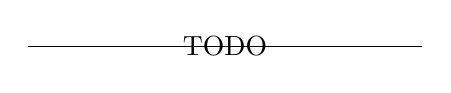
\begin{tikzpicture}
			\draw (0,0) rectangle (5,0) node[pos=.5] {TODO};
		\end{tikzpicture}
	\end{center}
	In the so-called \(N = 2\) dimensional \(\parentheses*{u_1, u_2}\) phase-space, the two initial points \(U_L\) and \(U_R\) are connected via the intermediate value \(U^*\) along the two directions determined by the eigenvectors \(\bm{r}_1, \bm{r}_2\) of \(A\).
	\begin{center}
		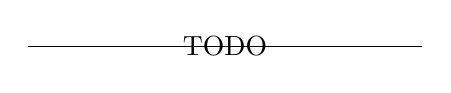
\begin{tikzpicture}
			\draw (0,0) rectangle (5,0) node[pos=.5] {TODO};
		\end{tikzpicture}
	\end{center}
\end{example}

The observations from the previous example can be extended to any linear Riemann problem.

\begin{theorem}[Linear Riemann solution]
	Consider a linear Riemann problem with flux \(F\parentheses*{U} = AU, A \in \R^{N \times N}\).
	Suppose that the initial jump satisfies
	\[
		U_R - U_L = \sum_{p = 1}^N \alpha_p \bm{r}_p
	\]
	for jump (or step) sizes \(\alpha_p \in \R, p = 1, \ldots, N\) with respect to the eigenvectors \(\braces*{\bm{r}_p}_{p = 1, \ldots, N}\) of \(A\).
	Then the unique Riemann solution of the linear PDE system
	\[
		\partial_t U + A\partial_x U = 0
	\]
	is given by \(N\) discontinuities with jumps \(\Brackets*{U}_p = \alpha_p \bm{r}_p\) and speeds \(s_p = \lambda_p, p = 1, \ldots, N\), and it holds that
	\[
		U\parentheses*{x, t} = U_L + \sum_{\frac{x}{t} > \lambda_p}\alpha_p \bm{r}_p = U_R - \sum_{\frac{x}{t} < \lambda_p}\alpha_p \bm{r}_p.
	\]
\end{theorem}

\begin{proof}
	Direct generalization of the \(2 \times 2\) example above; see, e.g., the book by LeVeque.
\end{proof}

\begin{remark}
	\begin{enumerate}
		\item As before, the jump is defined as \(\Brackets*{U} = U_{\text{after}} - U_{\text{before}}\) in the direction of the \(x\)-axis.
		\item In the \(\parentheses*{x, t}\)-diagram we have \(N\) rays for the \(N\) discontinuities.
		\item The discontinuities for the eigenvalue \(\lambda_p\) are called \emph{\(p\)-waves} or \emph{\(p\)-shocks}.
	\end{enumerate}
\end{remark}


\subsection{Nonlinear systems}

With our understanding of the linear Riemann problem we can now turn our attention to nonlinear systems.
That is, we consider general systems of conservation laws of the form
\[
	\partial_t U + \partial_x F\parentheses*{U} = 0, \quad \text{in }\R \times \parentheses*{0, \infty}.
\]

\begin{theorem}[General Riemann solution]
	A self-similar, weak entropy solution \(U\parentheses*{x, t} \in \R^N\) of the Riemann problem for \(t > 0\) of a nonlinear hyperbolic system of conservation laws os composed out of three different regions:
	\begin{enumerate}
		\item \emph{regions of constant values}
		\[
			U\parentheses*{x, t} = \text{const.},
		\]
		\item \emph{regions with (jump) discontinuities}
		\[
			U\parentheses*{x, t} = \begin{cases}
				U_1, & \text{if }x < st,\\
				U_2, & \text{if }x > st,
			\end{cases}
		\]
		with constant speed \(s\) that satisfies the Rankine-Hugoniot and entropy conditions,
		\item \emph{regions where the solution is differentiable}, that is, regions for which \(V\parentheses*{\xi} = V\parentheses*{\frac{x}{t}} = U\parentheses*{x, t}\) and its derivative \(V'\parentheses*{\xi} \equiv \partial_\xi V\parentheses*{\xi} \in \R^N\) satisfies
		\[
			\parentheses*{DF\parentheses*{V\parentheses*{\xi}} - \xi I}V'\parentheses*{\xi} = 0, \quad \xi = \frac{x}{t} \in \R,
		\]
		which are called \emph{rarefaction fans}.
	\end{enumerate}
\end{theorem}

\begin{proof}
	
\end{proof}
